\section{Interest Flooding Attacks in NDN}
\label{sec:interest-flooding}

% Points here:
% - Classification
% - Mechanisms: congestion and memory exhaustion
% - Target
% - Effectiveness: random names, non-existing content
% - Assumptions: the network, attackers, attack traffic, and legitimate consumers

%??? - References to the discussion about other types of attacks (ordifferent attack assumptions) about other attacks and explicitly stating that this work aims to build a baseline for general Interest Flooding mitigation problem, with other attack profiles and malicious gateways.

%\paragraph{What is it?}

Unlike Data packets, Interest packets in NDN are unsolicited, consume state in intermediate routers, and are routed through the network based on their content name prefix. These properties make Interest packets an effective tool in launching DoS and DDoS attacks in NDN. An attacker or a set of distributed attackers can inject excessive amounts of Interests to overload the network and cause service disruptions for legitimate users (Fig.~\ref{fig:flooding example}). 
%%% Alex %%% We have (almost) exactly the same sentence in the intro. I think here is kind of redundant, as it is obvious how we call the attack from the section title.  Also, we are referring to the term again in the last paragraph of the section.
% We coin the term \emph{Interest flooding} to refer to these network-level flooding attacks.

\begin{figure}[htbp]
  \centering
  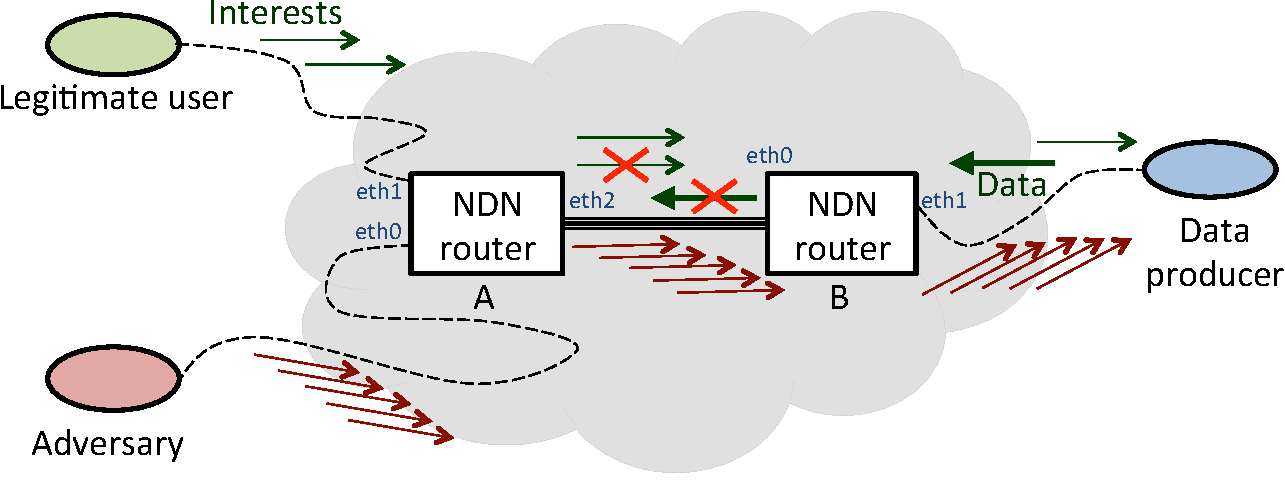
\includegraphics[scale=0.39]{attack-definition}
  \caption{Example of the Interest flooding attack}
  \label{fig:flooding example}
\end{figure}

%\paragraph{How does it work?}

Since communication in NDN is content-centric, it is unlikely that an adversary can target specific routers or end-hosts, as neither is required to have a globally routable network identity/address. However, an adversary can target a specific namespace.
For example in Fig.~\ref{fig:flooding example}, if the Data producer is the exclusive owner of \ndnName{/foo/bar} namespace, both router B and the Data producer would receive all Interests for \ndnName{/foo/bar/\ldots} that cannot be otherwise satisfied from in-network caches.%
\footnote {In our example, Data producer is single-homed. In the case of multi-homed producers with rich connectivity through multiple providers, NDN would likely to cope better with DDoS attacks due its native multipath and adaptive forwarding~\cite{adaptive-forwarding}.}
A large volume of these Interests can distrupt service quality in NDN network in two ways: \emph{create network congestion} and \emph{exhaust resources on routers}.

Similar to packets in traditional networks, Interest packets in NDN consume a portion of network capacity. A large number of Interest packets might cause congestion and lead to legitimate packets being dropped in the network. Although congestion might occur anywhere in the network, a coordinated DDoS attack would likely target one specific namespace to concentrate attack traffic in certain segments of the network, typically closest to the publisher serving that namespace since name prefixes in NDN loosely correspond to a network location or sets of network locations. 

As NDN routers maintain per-packet states for each forwarded Interest (i.e., an entry in its PIT), an excessive amount of malicious Interests can lead to exhaustion of a routers' memory. When a router has insufficient memory to create a new PIT entry, it is forced to drop new incoming Interests, thus disrupting service for legitimate users.
% there is no point in forwarding the Interest further.
% Otherwise, if Data comes back, it would be considered unsolicited and dropped anyways.
%Therefore, service for legitimate users can be disrupted due to limited memory resources in routers without saturating communication links to their limits.

%\paragraph{Target}


% \paragraph{Countermeasures}?

%\paragraph{Effectiveness}

To efficiently implement an Interest flooding attack targeting a specific namespace (e.g., \ndnName{/newyorktimes/}), an adversary needs to make sure that (1) the expressed Interests are routed as close to the Data producer as possible, and (2) the corresponding PIT entries are stored at intermediate NDN routers for as long as possible.
In order to achieve both requirements effectively, malicious Interests should avoid Interest collapsing and avoid being served from caches of intermediate routers: each malicious Interest generated by an individual attacker should request an unpopular or non-existing content, e.g., content with a unique name (\emph{unique junk Interests}). In this paper, we exclusively focus on this particular attack strategy as it maximizes the damage from each malicious Interest in the network. Other less effective strains of this attack can be mitigated by applying the same or similar countermeasures.  

In the rest of this paper, we use the general term \emph{Interest flooding attack} to refer to the above described attack and assume an attacker that is limited to controlling a botnet of end-hosts only, i.e., we assume the routers in the network and the computers in the victim domain are not compromised.

%\paragraph{Assumptions} 
%E: These are assumptions for the simulations on hand and particulary to test for the worst case scenario in many aspects. They are not the paper's assumption and in fact the paper first should be more general on describing all possibilities. Then it should explain the assumptions for the simulations and discuss why they make sense and do NOT favor positive results in some way. 

% - assumptions about attacker position
% - assumptions about the producer / producer namespace
% - assumptions about the attack traffic / attack pattern

%In this paper we are making the following assumptions about the Interest flooding attack:
%\begin{itemize}
%\item only client nodes can be compromised and become attack bots;
%\item there are no colluding attackers inside the Data producer's network;
%\item the attack is carried only using unique junk Interests; and
%\item there is only one Data producer for the attacked prefix.
%\end{itemize}

%We also assume that NDN forwarding strategy uses only single-path Interest forwarding, always choosing the best-metric route advertised by the routing protocol.
%This way, we are able to analyze the attack in its best environment, as enabling the multi-path forwarding would only alleviate effects of the Interest flooding attack.

%In section~\ref{sec:discussion} we discuss potential of the Interest flooding attack under several other attack assumptions.

%%% Local Variables: 
%%% mode: latex
%%% TeX-master: "paper"
%%% End: 
